\documentclass[a4paper,12pt]{article}
\usepackage[margin=0.25in]{geometry}
\usepackage{amsmath,amssymb,graphicx,ulem,fancyhdr,fix-cm,xcolor,soul}
\usepackage[utf8]{inputenc}
\usepackage[english]{babel}
\usepackage{xcolor}
\usepackage{lastpage}
\usepackage[english]{babel}
\usepackage{titlesec}

\titleformat{\section}[runin]
{\normalfont\Large\bfseries}{\thesection}{}{}

\definecolor{background}{rgb}{1,1,0.92}
\pagenumbering{arabic}
\graphicspath{ {./images/} }
\setlength\headheight{110pt} 
\pagestyle{fancy}

\begin{document}
\section*{}%Coverpage
%cover Page,w/ university logo
 \pagecolor{background}
 \fancyhead[R]{ 
\includegraphics[width=12cm]{logo.png}}
 \fancyhead[L]{\fontsize{15}{20} \selectfont \textbf{CSE 213 - Numerical Analysis\\ Spring '22\\ \ \\}}	
	\begin{center}
	\vspace*{6cm}
	\fontsize{40}{60} \selectfont Sheet 1 - Error Analysis \\
	\fontsize{30}{40}\selectfont CSE 213 - Numerical Analysis \\
	\fontsize{28}{35}\selectfont 120200033 \qquad \ CSE Section 01\\
	\fontsize{25}{30}\selectfont Ahmad Mongy Saad Aboelnaga\\
	\fontsize{20}{25}\selectfont Ahmad.Aboelnaga@ejust.edu.eg	
	\newpage
	\end{center}
	\addtolength{\topmargin}{-.75in}
	\fancyhead[R]{\Large \textbf{Sheet 1}}
	 \fancyhead[L]{\fontsize{18}{20} \selectfont CSE 213 - Numerical Analysis, Spring '22}
\section*{\LARGE Question 1:}

	\textbf{\Large Absolute and Relative Errors:} \Large If \(x\) is the exact value, and \(x^*\) is the approximate
value, calculate the absolute and relative errors when: 

	\begin{alignat*}{2}
 	a.\quad \    x &=& 10.147, x^* &= 10.159\\
 	b. \quad \   x &=& 0.0047, x^* &= 0.0045\\
 	c.  \quad \  x &=& 671000, x^* &= 669000 
	\end{alignat*}

{\color{blue}\textbf{Solution:}}

	\begin{align*}
 	\text{Absolute Error} &= { |\text{ Excat value } (x) - \text{ Approximate Value } (x^*)\text{ }|}\\
  	\text{Relative Error } &=  \frac{ |\text{ Excat value } (x) - \text{ Approximate Value } (x^*)\text{ }|}{\text{ Excat value } (x)}
	\end{align*}

{\color{red}\textbf{  \indent \(a.\)}}

	\begin{alignat}{3}
  	\text{Absolute Error \quad\ } &=& &| 10.147 -  10.159|& &= 0.012\\
  	\text{Relative Error \quad\ } &=&  &\frac{|10.147 - 10.159 |}{10.147}& &\approx 1.183\times 10^{-3}
	\end{alignat}
  
	{\color{red}\textbf{ \indent \(b.\)}}

 	\begin{alignat}{3}
  	\text{Absolute Error \quad\ } &=&  &| 0.0047 -  0.0045|& &= 0.0002 \\ 
  	\text{Relative Error \quad\ } &=&   &\frac{|0.0047 - 0.0045 |}{0.0047}& &\approx 4.255\times 10^{-2}
  	\end{alignat}
  

{\color{red}\textbf{  \indent \(c.\)}}
 \begin{alignat}{3}
  \text{Absolute Error \quad\ } &=&  &| 671000 - 669000 |& &= 2000 \\ 
  \text{Relative Error \quad\ } &=&   &\frac{|671000 - 669000 |}{671000}& &\approx 2.98\times 10^{-3}
  \end{alignat}
  
  
\newpage



\section*{\LARGE Question 2:}
	 \textbf{\Large Truncation Error:}
	 Use only the first 3 terms of the series
	 
	 \begin{align*}
		sin(x) = \sum_{i=0}^{\infty} (-1)^i \dfrac{x^{2i+1}}{(2i+1)!}
	 \end{align*}
	 
	 to evaluate \(sin(\dfrac{\pi}{2})\) and then find the truncation error.\\[0.5cm]
	{\color{blue}\textbf{Solution: \\[0.5cm]}}
	\indent{The Exact Value of \(sin(\dfrac{\pi}{2}) = 1\) \\
	\indent{ Using only the first 3 terms of the series we get: }}
	\begin{alignat*}{4}
		sin(\dfrac{\pi}{2}) &=& &(-1)^0 \dfrac{\dfrac{\pi}{2}^{2 \times 0 +1}}{(2\times 0 +1)!}& &+(-1)^1 \dfrac{\dfrac{\pi}{2}^{2 \times 1 +1}}{(2\times 1 +1)!}& &+(-1)^2 \dfrac{\dfrac{\pi}{2}^{2 \times 2 +1}}{(2\times 2 +1)!}\\ 
		&=& &+1.5707963& &-0.6459641& &+0.0796926\\
		&=& &+1.0045248\\
	\end{alignat*}
	
\paragraph*{\Large Truncation Error:}
	\begin{alignat*}{2}
		R_3(X)&=& |1-1.0045248|  &= 0.0045248 \quad \qquad  \text{(Absloute Error)} \\
		\therefore \text{Truncation Error }&=& \dfrac{0.0045248}{1} &= 0.45248\times 10^{-2} \quad \text{(Relative Error)}
	\end{alignat*}

\newpage




\section*{\LARGE Question 3:}
 \textbf {\Large Hypothetical Machine:}
 Consider a hypothetical digital computer in which the binary representation of a real number is: (1)(001)(11010), where (001)
corresponds to the Exponent, and (11010) corresponds to the Mantissa. Find:
 \begin{flushleft}
a. The values of the parameters L, U, p, and b.\\
b. The representation (in base 10) of the given binary representation.\\
c. The absolute error resulting from the operation: 1.75 – 0.1875\\
d. The Maximum and Minimum decimal values that can be represented by the given machine.\\
e. How many different numbers are in this floating point system?
 \end{flushleft}
 {\color{blue}\textbf{Solution: \\}}
 \indent{\color{red}a)}
 \begin{align*}
 \text{L} &= -(11)_2 =-(3)_{10} \quad \text{(one bit for sign and two bit for the value),} \\
 \text{U} &= +(11)_2 =+(3)_{10} \quad \text{(Upper limit)},\\
 \text{b} &= 2 \qquad \qquad \qquad \qquad \text{(Binary Base)},\\
 \text{p} &= 5 \qquad \qquad \qquad \qquad \text{(Length of mantissa)}
 \end{align*} 
 \indent{\color{red}b)}
 \begin{alignat*}{3}
 &(\color{red}1\color{green}001\color{blue}11010\color{black})\\
 &\color{red}\downarrow\color{green}\downarrow\downarrow\downarrow\color{blue}\downarrow\downarrow\downarrow\downarrow\downarrow\\
 &\color{red}-\color{green}2^{1}\color{black}\times\color{blue}(2^{-1}+2^{-2}+2^{-4})\color{blue}\\
 &=(-1.625)_{10}
 \end{alignat*}
  \indent{\color{red}c)}
 \begin{alignat*}{2}
 x  &=& 1.75 - 0.1875 &= 1.5625 \quad \text{(The exact value)}\\
 x^*&=& \texttt{fl}\left(\texttt{fl}(1.75)-\texttt{fl}(0.1875)\right) &=1.5625 \quad \text{(The machine value)}
  \end{alignat*}
   \indent \qquad $\therefore$ \text{Absloute Error} = \(|x - x^*|\) = $0$\\[0.2cm]
	\texttt{fl}(1.75)$\rightarrow$ (0)(001)(11100), has an exact representation\\
	\texttt{fl}(0.1875)$\rightarrow$ (0)(110)(11000), has an exact representation\\
	\texttt{fl}(1.5625)$\rightarrow$ (0)(001)(11001), has an exact representation\\
 \newpage
 \indent{\color{red}d)}\\
 \indent \qquad Min -ve Value at (1)(011)(11111)=-7.75,\\
 \indent \qquad Min +ve Value at (0)(111)(10000)=+0.0625,\\
 \indent \qquad Max +ve Value at (0)(011)(11111)=+7.75\\[1cm]
 \indent{\color{red}e)} Possible combinations in
 \begin{itemize}
 	\item \indent sign-bit =2  [(0),(1)]
 	\item exponent =7 [(000),(001),(010)...]
 	\item mantissa =16 [(10000),(10001)...]
 \end{itemize}
 \indent \quad Total possible numbers that can be represented in this machine\\
 \indent \quad $= 2\times 7 \times 16 $\\
 \indent \quad $= 224\,$ different numbers

\newpage
\section*{\LARGE Question 4:}
 Verify that the chopping error resulting from calculating\\
 $(1.0/6.0)$ to 2 significant digits will cause that $(1.0/6.0) \times 6.0 \neq 1.0$. Verify that when $(1.0/6.0)$ is
approximated to 5 decimal digits, the result of $(1.0/6.0) \times 6.0$ will be 0.99996\\[0.5cm]
 {\color{blue}\textbf{Solution: \\[0.4cm]}}
 \indent{$\dfrac{1.0}{6.0} \approx 0.16$ chopped at 2 significant digits}\\[0.4cm]
\indent $\therefore (1.0/6.0) \times 6.0 \rightarrow 0.16 \times 6.0 =0.96 \neq 1.0$\\[0.4cm]
\indent{$\dfrac{1.0}{6.0} \approx 0.16666$ chopped at 5 significant digits}\\[0.4cm]
\indent $\therefore (1.0/6.0) \times 6.0 \rightarrow 0.16666 \times 6.0 = 0.99996$ 

\newpage
\section*{\LARGE Question 5:}
 The critical part of floating-point operations is the potential loss of correct digits in the significand. Consider a computer model that uses 4 digits for the significand, 1 digit for the exponent plus an optional sign for both the significand and the exponent, any real number 'a' may be written as a normalised decimal number a$\times10^n$, where the number 'a' is in the range [0.1,1) and is called the significand, while the the integer n is called the exponent.\\
Convert the following numbers to normal form and perform the required operation:
 \begin{flushleft}
$1)\,a = 42.34$ and $b = 0.0033$, calculate $a+b$\\
$2)\,a = 10.34$ and $b =-10.27$, calculate $a+b$\\
$3)\,a = 10/7$ and $b =-1.42$, calculate $a+b$\\
$4)\,a = 23.57$ and $b =-6.759$, calculate $a*b$ and $a/b$
 \end{flushleft}
 {\color{blue}\textbf{Solution: \\}}
 \indent{$1)\,a=42.34,\quad \textit{fl}(a)\rightarrow 0.4234\times 10^2$}\\
 \indent{\quad{$b=0.0033,\quad \textit{fl}(b)\rightarrow 0.3300\times 10^{-2}$}}\\
 \indent {\quad $a+b= 0.423433\times 10^2, \quad \textit{fl}(a+b)\rightarrow 0.4234\times 10^2\, \text{(Normalized)}$} \\[0.5cm]
  \indent{$2)\,a=10.34,\quad \textit{fl}(a)\rightarrow 0.1034\times 10^2$}\\
 \indent{\quad{$b=-10.27,\quad \textit{fl}(b)\rightarrow -0.1027\times 10^2$}}\\
 \indent {\quad $a+b= 0.0007\times 10^2 \quad \textit{fl}(a+b)\rightarrow 0.7000\times 10^{-1}\, \text{(Normalized)}$} \\[0.5cm]
  \indent{$3)\,a=10/7,\, \textit{fl}(a)\rightarrow 0.1428\times 10^1 \text{ chopped or }0.1429\times 10^1 \text{ rounded } $}\\
 \indent{\quad{$b=-1.42,\, \textit{fl}(b)\rightarrow -0.1420\times 10^1$}}\\
 \indent {\quad $a+b\approx 8.571428\times 10^{-3},\quad \textit{fl}(a+b)\rightarrow 0.8\times 10^{-2}\text{ chopped or }0.9\times 10^{-2}\, \text{rounded}$} \\[0.5cm]
   \indent{$4)\,a=23.57,\quad \textit{fl}(b)\rightarrow 0.2375\times 10^2$}\\
 \indent{\quad{$b=-6.759,\quad \textit{fl}(b)\rightarrow -0.6759\times 10^1$}}\\
 \indent {\quad $a*b= -1.5931\times 10^2 \quad \textit{fl}(a*b)\rightarrow -0.1593 \times 10^{3}\, \text{(Normalized by rounding)}$} \\
  \indent {\quad $a/b= -0.34872\times 10^1 \quad \textit{fl}(a/b)\rightarrow -0.3487 \times 10^{1}\, \text{(Normalized)}$} \\
\newpage

\section*{\LARGE Question 6:}
\textbf{Consider the simple algorithm:\\}
$x = 0.0;$\\
\textbf{while} $x \neq 1.0$\\
\indent \textbf{print} $x$\\
\indent $x = x +0.1;$\\
Implement the algorithm in a program and check what values of x will be printed?
Explain what happened.\\[0.5cm]
 {\color{blue}\textbf{Solution:\\[0.2cm]}}
 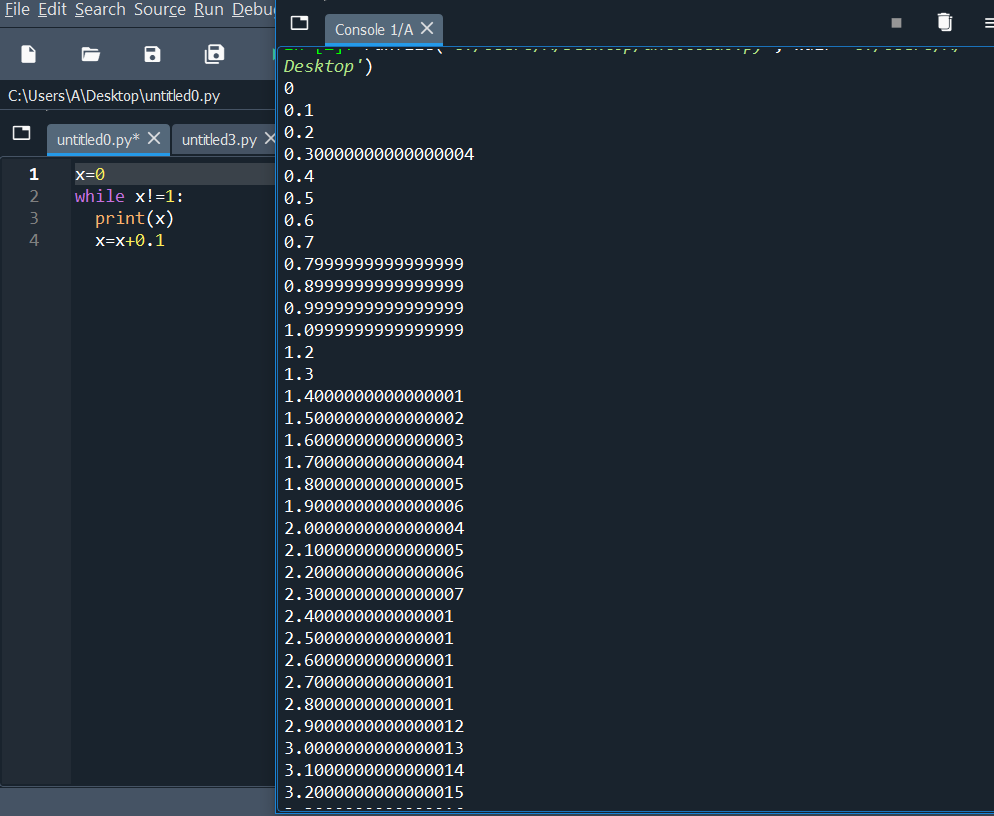
\includegraphics[width=20cm]{Q6.png}
 As 0.1 does not have a finite representation in binary,there is an approximation error and it shows for example in 0.3 as the machine prints 0.30000000000000004 instead. Due to the error of finite representation an exact 1 is never reached and there for the program enters an infinite loop and continue printing numbers that is greater than 1.
\newpage

\section*{\LARGE Question 7:}
The following Python program shows the effect of the propagation of an initial representation error which results in final (large!) error. Run the program, print its results once for k in range(10) and in range(30). Comment on the obtained results.\\
a=[  ]\\
for n in range (1,11)\\
\indent {x= 1/n} \\
\indent {for k in range (30):}\\
\indent {\indent {x=(n+1)*x-1}}\\
\indent {a.append(x)}\\
print(a)\\[0.5cm]
 {\color{blue}\textbf{Solution: \\[0.3cm]}}
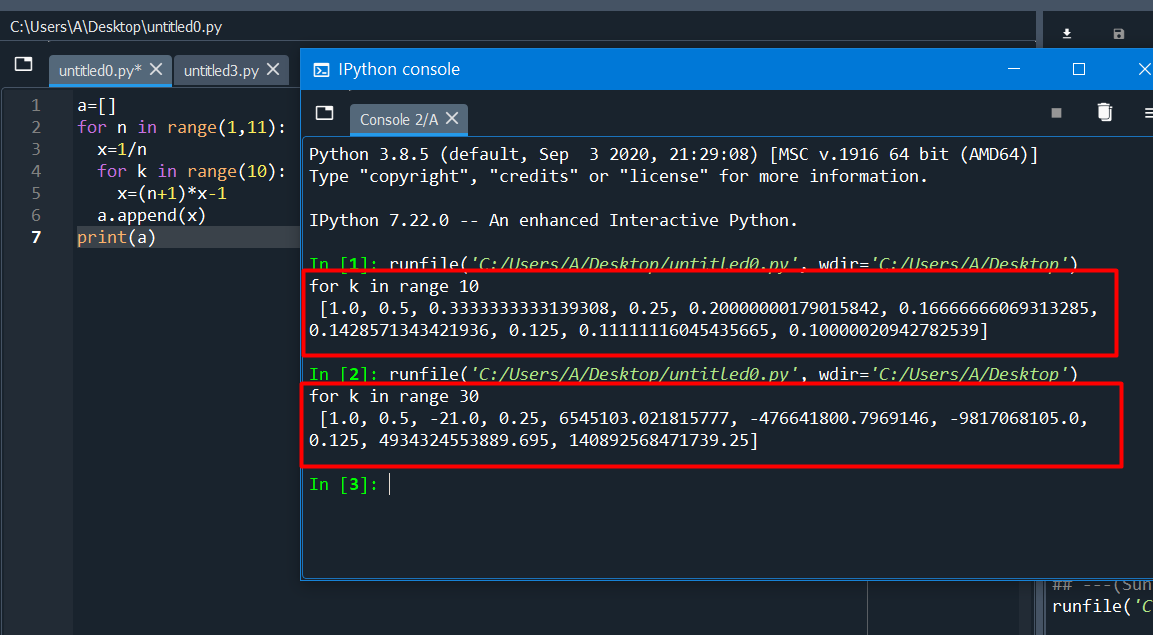
\includegraphics[width=20cm]{Q7.png}
As there are approximation errors due to machine finite representation, these errors propagate through the iterations and therefore present a solution with larger error, and this can be observed for all numbers that does not have an exact representation in the machine
\newpage




\section*{\LARGE Question 8:}
\emph{\textbf{Errors in Computer Arithmetic}}\\
In order to reduce the chance of large errors occurring in calculations, here are some tips that you should consider:\\[0.5cm]
i. In general, it is better to add ‘floating-point’ numbers in order of magnitude if possible. For example, suppose we compute
$0.273000+0.001480+0.000862 (=0.275342).$ If results are stored with mantissas 3 digits long; then,\\[0.2cm]
$0.273000 + 0.001480 = 0.274480  \rightarrow 0.274000$ and\\[0.2cm]
$0.27400 + 0.000862 = 0.274862  \rightarrow 0.274000$\\[0.2cm]
whereas\\[0.2cm]
$0.000862 + 0.001480 = 0.002342  \rightarrow 0.002340$ and\\[0.2cm]
$0.002340 + 0.27300 = 0.275340  \rightarrow 0.275000$\\[0.2cm]
ii. In order to prevent ‘loss of significance’, it is important to avoid a ‘bad subtraction’ that is, a subtraction of a number from another number having almost equal value. Let us consider a simple problem of finding the roots of a second-order equation $ax^2 + bx +c=0$ by using the formulas:
 \[x_1= \dfrac{-b+\sqrt{b^2-4ac}}{2a},\qquad x_2= \dfrac{-b-\sqrt{b^2-4ac}}{2a}\]
 Assuming the Discriminant: $b^2 - 4ac > 0$, then depending on the sign of b, a “bad subtraction” may be encountered when we try to find the smaller one of the two roots. This implies that it is safe, from the “loss of significance” point of view, to compute the root having the larger absolute value first and then obtain the other root by using the relation (between the roots and the coefficients) $x_1x_2= c/a$.\\[0.3cm]
 a) Apply this technique to solve the equation $x^2 + 62.10 x + 1 = 0$ whose roots are
Approximately : $x_1 = -0.01610723$ and $x_2= -62.08390$. Check the relative errors in the obtained roots (using four-digit rounding arithmetic) in case of finding both roots using the formulas and the case of avoiding "bad subtraction".\\[0.4cm]
b) Apply the idea of rationalizing the numerator of the quadratic formula to obtain a more accurate four-digit rounding approximation for $x_1$
\[x_1 = \dfrac{-b+\sqrt{b^2-4ac}}{2a} \left(\dfrac{-b-\sqrt{b^2-4ac}}{-b-\sqrt{b^2-4ac}} \right)= \dfrac{b^2 - (b^2-4ac}{2a(-b-\sqrt{b^2-4ac})}\]
\newpage
$ \quad \qquad = \dfrac{-2c}{b+\sqrt{b^2-4ac}}$\\[0.3cm]
iii. In consecutive multiplication/division processes, make the intermediate result as close to one as possible. According to this rule, when computing $xy/z$, we program the formula as:
\begin{itemize}
\item $(xy)/z$ when $x$ and $y$ in the multiplication are very different in magnitude,
\item $x(y/z)$ when $y$ and $z$ in the division are close in magnitude, and 
\item $(x/z)y$ when $x$ and $z$ in the division are close in magnitude.
\end{itemize} 
For instance, when computing $y^n/e^{nx}$ with $x>1$ and $y>1$, we would program it as $(y/e^x)^n$ rather than as $y^n/ e^{nx}$ , so that overflow/underflow can be avoided. Verify this using Excel/ Python/ Matlab for the case:\\
x = 36; y = 1e16; for n = {-20, -19, 19, 20}.\\[0.5cm]
{\color{blue}\textbf{Solution: \\}}
 \indent{\color{red}a \& b) \color{black}$a=1,\,b=62.10,\,c=1$}\\
 \indent \quad{$a=0.01\times 10^2 ,\, b=0.6210 \times 10^2,\,c=0.100\times 10^2$}\\
 \indent\quad $x_2 =-62.08$, using root formula\\
 \indent\quad For $x_1$:\\[0.3cm]
 \begin{tabular}{|c|c|c|c|}
 \hline 
 Method & Using root Formula & Avoid Bad Subtrac & Ration Numerator \\ 
 \hline
 $X_1$ Value & $-0.02\times 10^0$ & $-0.01611$ & $-0.01611$ \\
 \hline 
 Abs Error(e)& $3.89277\times 10^{-3}$ & $2.77\times 10^{-6}$ & $2.77\times 10^{-6}$ \\ 
 \hline 
 Relative Error(r) & $0.24168$ & $1.7197\times 10^{-4}$ & $1.7197\times 10^{-4}$ \\ 
 \hline 
 \end{tabular}\\[0.3cm]
 
 \indent{\color{red}iii)}\color{black} As show in the figure in next page, the result of using both algorithms have yielded close results with one of them having more accurate calculation each time, moreover, in the case with n=20 the second method ($y^n/e^{nx}$) has resulted in Over Flow Error, while the other method ($(y/e^x)^n$) returned a result
 \newpage
 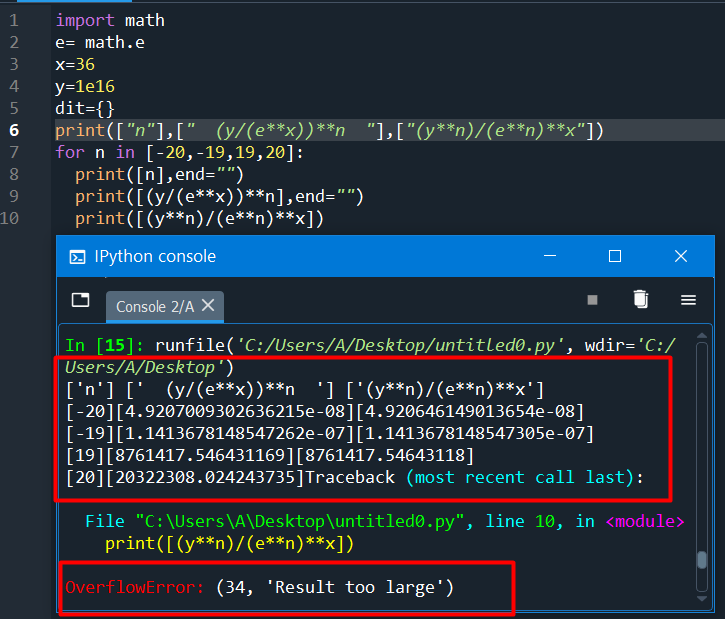
\includegraphics[scale=1.4]{Q8.png}\\[2cm]
 Tools used in creating this document:
 \begin{itemize}
 \item Texmaker 5.0.4
 \item Spyder IDE 5.1.5 with python 3.8.5
\end{itemize}  
 
 \copyright All questions in this file has been adapted from the sheet provided by the course instructor, I have only reorganized the sheet and attempted to answer it. Please do not share without the permission of the owner.\\
Thanks for my colleagues who helped me reviewing the file\\
\color{blue}Ahmad.Aboelnaga@ejust.edu.eg\\
ID:120200033, CSE01
 
  
\end{document}			
